\documentclass[10pt,twocolumn]{article}
\usepackage[letterpaper,margin=0.75in,columnsep=0.25in]{geometry}
\usepackage{libertinus}
\usepackage{microtype}
\usepackage{titlesec}
\titlespacing*{\paragraph}{0pt}{5pt plus 2pt minus 1pt}{0.6em}
\titleformat{\paragraph}[runin]{\normalfont\bfseries}{}{0pt}{}
\usepackage{booktabs}
\usepackage{longtable}
\usepackage{tabularx}
\usepackage{array}
\usepackage{multirow}
\usepackage{xcolor}
\usepackage{caption}
\usepackage{subcaption}
\usepackage{enumitem}
\usepackage{amsmath}
\usepackage{pgfplots}
\usepackage{tikz}
\usetikzlibrary{positioning,arrows.meta,fit,backgrounds,calc}
\pgfplotsset{compat=1.18}
\usepackage[hidelinks]{hyperref}
\usepackage{cleveref}

\definecolor{hs}{HTML}{1F4E79}
\definecolor{hg}{HTML}{B4B4B4}
\definecolor{rule}{HTML}{555555}

\captionsetup{font=small,labelfont=bf,skip=4pt}
\setlist{nosep,leftmargin=1.2em}
\setlength{\tabcolsep}{4pt}
\renewcommand{\arraystretch}{1.08}
\frenchspacing

\newcommand{\wl}[1]{\texttt{#1}}
\newcommand{\M}[1]{\csname #1\endcsname}
\newcommand{\hstore}{HStore}
\newcommand{\hgdb}{HyperGraphDB}

\pgfplotsset{
  report/.style={
    font=\footnotesize,
    tick label style={font=\scriptsize},
    label style={font=\footnotesize},
    legend style={font=\scriptsize,draw=none,fill=none},
    axis line style={rule},
    tick style={rule},
    major grid style={gray!25},
  },
}

\input{gen/macros}
\input{gen/summary-fig}

\title{\Large\bfseries HStore and HyperGraphDB:\\ a storage-level benchmark of two persistent hypergraph engines}
\author{Metacog Labs\\[2pt]\normalsize HStore 0.1.0, commit \texttt{459b8be}}
\date{October 2026}

\begin{document}
\maketitle

\begin{abstract}
We compare HStore, a persistent hypergraph storage engine built on copy-on-write counted B+trees, with HyperGraphDB~1.4 on Berkeley DB Java Edition. Both systems run 26 storage-level workloads on the same skewed synthetic hypergraph, with up to 1.45 million incidences and equal 64\,MiB caches, in three configurations: two data sizes and two commit modes. Every read result is cross-checked between the systems. At scale 1 with asynchronous commits, HStore enumerates incidence sets \M{ratioAreadincidence} faster, counts shared hyperedges \M{ratioAreadcomembership} faster, applies batched updates \M{ratioAwriteupdate} faster, and needs \M{ratioAdisk} less disk. These leads come from storing incidence sets as small sorted trees, and from commits that log only the keys they changed while a background checkpoint writes pages. When the data is four times larger than the cache, HStore keeps most of these leads but falls to \M{sumCreadmembers} of HyperGraphDB's speed on member enumeration, because its member lookups miss the node cache. With synchronous commits, both systems are bound by the cost of one forced write per commit. We also report latency percentiles, bytes written, heap use, space reclamation and crash recovery, the variation over runs, and a durability setting in HyperGraphDB that, left unchecked, makes its synchronous commits unsynced.

\end{abstract}

\section{Introduction}

Many datasets record facts that involve more than two things at once. An insurance claim joins a patient, a provider, a drug and a pharmacy. A paper joins its authors, and a meeting joins its participants. A hypergraph stores each such fact as one hyperedge over all of its participants. A property graph has to break the same fact into a new node and one edge per participant, and a relational schema into a join table. Queries then ask hypergraph questions: which facts involve this entity, which facts involve both of these entities, and what lies two hops away.

HyperGraphDB~\cite{hgdb} is the established open-source hypergraph database for the JVM. It stores atoms and links in Berkeley DB Java Edition (JE), a general-purpose log-structured key-value store. HStore is a newer engine built for this data model. Its incidence sets and hyperedge memberships are counted B+trees, and its storage, transaction and recovery design is described in \cref{sec:systems}.

This report compares the two systems at the storage level, on the same machine and data, with the same cache budget. We measure what an embedded application sees: throughput of loads, updates, deletes and reads; per-operation latency, including tail latency while another thread writes; behaviour of giant hyperedges; disk footprint before and after deletes and space reclamation; time to recover after a crash; and the bytes written, heap allocated and GC time behind each result. Every read result is cross-checked between the two systems.

\Cref{sec:method} describes the dataset, workloads and measurement method. \Cref{sec:results} presents the results, and \cref{sec:discussion} explains them in terms of each system's design. \Cref{sec:validity} lists the limits of this study. Full tables, per-run values and the steps to reproduce every number are in the appendices.

\paragraph{Summary of findings.}
\begin{itemize}
\item \textbf{Incidence-based reads} are faster in HStore in every configuration: \M{sumCreadincidence} to \M{sumAreadincidence} for incidence sets, \M{sumCreadcomembership} to \M{sumBreadcomembership} for co-membership counts, and \M{sumCreadincidencecold} to \M{sumAreadincidencecold} directly after a reopen.
\item \textbf{Writes} cost HStore far fewer bytes. Single-update commits write \M{bpoAhstorelatencycommit} against \M{bpoAhgdblatencycommit}, and batched updates run \M{sumBwriteupdate} to \M{sumCwriteupdate} faster. Bulk insertion is closer: between \M{sumBingestedges} and \M{sumCingestedges} for hyperedges.
\item \textbf{Member enumeration} is HStore's weakness once the data outgrows its node cache: \M{sumCreadmembers} at scale 4, and \M{sumCreadtwohop} for two-hop neighbourhoods, which depend on it.
\item \textbf{Tail latency.} HStore's p99 and p99.9 latencies are lower than HyperGraphDB's in every latency workload and configuration, by 1.3 to 69 times. The single slowest commit at scale 4 was HStore's.
\item \textbf{Disk.} HStore's files are \M{sumBdisk} to \M{sumCdisk} smaller after loading. After deletes they first grow while retained history still references the replaced pages.
\item \textbf{Recovery.} Neither system lost an acknowledged commit after SIGKILL. Recovery times overlap.
\end{itemize}


\section{Systems under test}
\label{sec:systems}

Both systems are embedded Java libraries. Each runs in its own JVM process, and the benchmark harness calls its API directly. Neither is accessed over a network.

\subsection{HStore}

\paragraph{Data model.} Every stored object is an \emph{atom} with a 64-bit identifier. An atom is a node or a hyperedge. A hyperedge has any number of members, and a member can itself be a hyperedge. Hyperedges are either \emph{set} edges, keyed by member, or \emph{ordered} edges, keyed by position. Each membership carries a role set, a weight, a validity interval and a qualifier. The benchmark uses set edges and plain memberships.

\paragraph{Layout.} All persistent state is held in copy-on-write counted B+trees. Every child reference stores a summary of its subtree: the entry count, the key range and an order-independent fingerprint. Three trees matter here:
\begin{itemize}
\item The \emph{catalog} maps an atom id to its record. A hyperedge record holds a reference to that edge's \emph{membership tree}, keyed by member id. If the membership tree is one leaf of at most 32 entries that fits in about 100 bytes, it is stored inside the record itself and needs no page of its own.
\item The \emph{reverse incidence index} maps an atom id to the set of hyperedges that contain it. Sets of up to 48 entries are stored inline in the index leaf. Larger sets are promoted to a tree of their own.
\item Secondary indexes on node keys and properties, which the benchmark touches only through node insertion and updates.
\end{itemize}
Enumerating an incidence set is a cursor walk over one inline list or one small tree. Counting the hyperedges that contain two given atoms is a leapfrog intersection~\cite{leapfrog} of their two incidence trees. The intersection skips whole subtrees whose key range cannot contain a match.

\paragraph{Pages and files.} A tree node is written as a self-describing image: an 80-byte header with a CRC32C checksum, followed by the payload. Images are packed into append-only segment files of 256\,MiB, aligned to 64-byte units. A page directory maps each page number to the image's current address, so compaction can move an image without rewriting the trees that refer to it. Reads go through a memory map of each segment. Decoded nodes are kept in a node cache whose budget is set in bytes.

\paragraph{Generations and readers.} A committed state is a \emph{generation}: an immutable vector of tree roots. A reader pins a generation and reads it without locks. Writers never modify a node that a published generation can reach, as in other copy-on-write B+tree stores~\cite{lmdb}. The last 64 generations are retained for time travel.

\begin{figure*}[t]
\centering
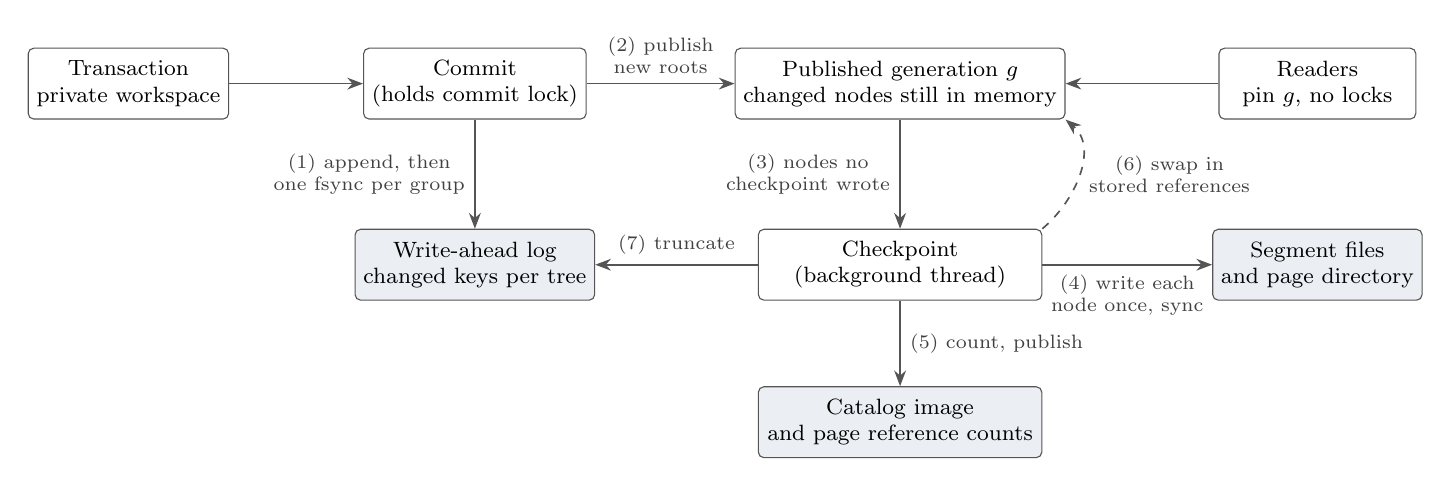
\begin{tikzpicture}[
  font=\footnotesize,
  box/.style={draw=rule,rounded corners=2pt,minimum height=9mm,minimum width=25mm,inner sep=3pt,align=center,fill=white},
  disk/.style={box,fill=hs!9},
  arr/.style={-{Stealth[length=2mm]},rule,semithick},
  lab/.style={font=\scriptsize,align=center,text=black!75}]
\node[box] (txn) at (0,0) {Transaction\\private workspace};
\node[box] (commit) at (4.4,0) {Commit\\(holds commit lock)};
\node[box,minimum width=36mm] (gen) at (9.8,0) {Published generation $g$\\changed nodes still in memory};
\node[box] (read) at (15.1,0) {Readers\\pin $g$, no locks};
\node[disk] (wal) at (4.4,-2.3) {Write-ahead log\\changed keys per tree};
\node[box,minimum width=36mm] (ckpt) at (9.8,-2.3) {Checkpoint\\(background thread)};
\node[disk] (seg) at (15.1,-2.3) {Segment files\\and page directory};
\node[disk,minimum width=36mm] (cat) at (9.8,-4.3) {Catalog image\\and page reference counts};
\draw[arr] (txn) -- (commit);
\draw[arr] (commit) -- node[lab,above]{(2) publish\\new roots} (gen);
\draw[arr] (read) -- (gen);
\draw[arr] (commit) -- node[lab,left]{(1) append, then\\one fsync per group} (wal);
\draw[arr] (gen) -- node[lab,left]{(3) nodes no\\checkpoint wrote} (ckpt);
\draw[arr] (ckpt) -- node[lab,below]{(4) write each\\node once, sync} (seg);
\draw[arr] (ckpt) -- node[lab,right]{(5) count, publish} (cat);
\draw[arr] (ckpt) -- node[lab,above]{(7) truncate} (wal);
\draw[arr,dashed] (ckpt.north east) to[out=40,in=-40] node[lab,right]{(6) swap in\\stored references} (gen.south east);
\end{tikzpicture}
\caption{HStore's write path. (1, 2) A commit logs only the keys it changed and publishes new roots whose changed nodes are still in memory. (3--7) A background checkpoint writes those nodes to pages, once for all the commits since the previous checkpoint, then swaps the stored references into the current generation and truncates the log. Only step 6 takes the commit lock.}
\label{fig:writepath}
\end{figure*}

\paragraph{Commits and checkpoints.} \Cref{fig:writepath} shows the write path. A transaction collects its changes in a private workspace. At commit it applies them to new copies of the affected tree paths, appends one write-ahead log record listing the keys it changed in each tree, and publishes the new generation. The new tree nodes stay in memory, reachable from the published roots. A background checkpoint later writes every node that no earlier checkpoint wrote, syncs the files, updates page reference counts, and publishes a catalog image. It then swaps the stored references into the current generation and truncates the log. Only the swap holds the commit lock. Memory held by unwritten nodes is capped at 64\,MiB. A commit that finds the cap reached waits for a checkpoint.

Two exceptions write pages before the checkpoint. A large bulk load spills finished subtrees to pages while it runs, and a tree that changed in more than 4,096 places is written to pages at commit and logged by reference. Under \emph{synchronous} durability, a commit returns after its log record is fsynced; concurrent commits share one fsync (group commit). Under \emph{asynchronous} durability the fsync is skipped, but commits are still published strictly in order.

\paragraph{Recovery.} On open, HStore loads the newest catalog image and replays the logged key changes of every commit after it, in commit order. A commit's changes are applied only if its commit record reached the log, so recovery always yields a prefix of the commit order.

\paragraph{Space reclamation.} Every page has a reference count, which changes only at checkpoints. A page no generation can reach is released once no pinned reader can see it. A segment whose live bytes fall below half of the bytes written to it is compacted: its live images are copied to the active segment, the page directory is updated, and the old file is deleted once no reader can still be using it. A background maintenance pass, run every 500\,ms, compacts one such segment at a time. An explicit compaction request compacts all of them.

\subsection{HyperGraphDB}

HyperGraphDB~\cite{hgdb} is a general hypergraph database for Java. Its atoms are identified by persistent handles (UUIDs). A link stores the ordered array of its target handles. The benchmark uses \texttt{HGPlainLink} for hyperedges and \texttt{String} atoms for nodes. The incidence set of an atom, the links pointing to it, is maintained by HyperGraphDB in a separate index. The atom cache keeps recently used atoms and incidence sets in memory as Java objects.

We use the Berkeley DB Java Edition storage implementation (\texttt{bdb-je}), the default for HyperGraphDB~1.4. JE is a log-structured B+tree store~\cite{je,lfs}: every update appends a new version of the changed records and internal nodes to the log. A background cleaner copies the live entries out of underused log files and deletes them. A checkpointer bounds recovery time. Incidence sets are stored as sorted duplicate sets in a JE database. A lookup opens a cursor at the atom's handle.

\subsection{Synchronous commits in HyperGraphDB}
\label{sec:durability}

HyperGraphDB 1.4 begins every JE transaction with an explicit \texttt{WRITE\_NO\_SYNC} durability. That setting overrides the environment-wide \texttt{COMMIT\_SYNC}, so configuring the environment alone leaves commits unsynced: in a first run of the synchronous configuration, HyperGraphDB committed single updates in about 0.1\,ms, while one forced write on this machine takes about 3.8\,ms. For the synchronous configuration the HyperGraphDB adapter therefore calls \texttt{Environment.flushLog(true)} after every commit. This writes and forces JE's log, which is what \texttt{COMMIT\_SYNC} would do at commit time. The asynchronous configuration is unaffected.

\subsection{Versions and configuration}

\Cref{tab:config} lists the configuration of both systems. The two caches are given the same 64\,MiB budget. HStore's budget covers decoded nodes. JE's budget covers its B+tree nodes and records, and HyperGraphDB's atom cache comes on top of it. That cache is sized by HyperGraphDB itself and cannot be capped in bytes. The retained-heap figure in \cref{sec:resources} shows what each store actually kept.

\begin{table*}[t]
\centering\footnotesize
\caption{System configuration. Both systems use their defaults except where stated.}
\label{tab:config}
\begin{tabularx}{0.82\textwidth}{@{}lXX@{}}
\toprule
& \hstore & \hgdb \\
\midrule
Version & 0.1.0, commit \texttt{459b8be}, storage format 7 & 1.4, commit \texttt{99485a1}; JE 5.0.73 \\
Cache & node cache, 64\,MiB & JE cache 64\,MiB, plus atom cache \\
Async commits & no fsync, ordered publication & JE \texttt{WRITE\_NO\_SYNC} (default) \\
Sync commits & fsync per commit group & JE log forced after each commit (\cref{sec:durability}) \\
Page / node size & 16\,KiB pages & JE defaults \\
Space reclamation & compact segments below 50\% live & cleaner, 50\% minimum utilisation \\
History & 64 generations & none \\
\bottomrule
\end{tabularx}
\end{table*}

\section{Benchmark design}
\label{sec:method}

\subsection{Dataset}

The dataset is generated from a fixed seed (20260904), so both systems load exactly the same graph. At scale $s$ it has $50{,}000\,s$ nodes and $100{,}000\,s$ hyperedges. The cardinality of a hyperedge follows a geometric tail: it starts at 2 and each further member is added with probability 0.62, up to 32, for a mean of 3.6. Members are drawn as $\lfloor n\,u^{2.2}\rfloor$ for uniform $u\in[0,1)$ over $n$ nodes. Low-numbered nodes therefore become hubs with large incidence sets, as in co-authorship, claims or citation data. Hyperedges never repeat a member.

\begin{table}[t]
\centering\footnotesize
\caption{Dataset statistics, computed from the generator. An incidence set is the set of hyperedges that contain a node.}
\label{tab:dataset}
\begin{tabular}{@{}lrr@{}}
\toprule
& Scale 1 & Scale 4 \\
\midrule
Nodes & 50{,}000 & 200{,}000 \\
Hyperedges & 100{,}000 & 400{,}000 \\
Incidences & 362{,}757 & 1{,}453{,}427 \\
\midrule
Hyperedge cardinality, mean / p99 / max & 3.63 / 11 / 30 & 3.63 / 11 / 30 \\
Incidence set size, mean & 7.26 & 7.27 \\
Incidence set size, p50 / p90 / p99 & 5 / 12 / 41 & 5 / 13 / 42 \\
Incidence set size, p99.9 / max & 145 / 2{,}645 & 142 / 5{,}714 \\
Nodes in no hyperedge & 575 & 2{,}319 \\
Incidence sets above 48 entries & 370 & 1{,}521 \\
\bottomrule
\end{tabular}
\end{table}

\Cref{tab:dataset} gives the sizes and the skew. The largest incidence set at scale 1 holds 2,645 hyperedges, while half of all nodes are in 5 or fewer. Only 370 incidence sets exceed the 48 entries that HStore stores inline. Probe sets drawn from the same seed hold 100,000 random nodes and hyperedges, 20,000 node pairs taken from a common hyperedge (so that co-membership counts are non-zero), and 20,000 node updates. A separate churn set, drawn after everything else, selects 20\% of the hyperedges for deletion and 20,000 other hyperedges, each with at least three members, that lose one member.

\subsection{Workloads}

\Cref{tab:workloads} defines the workloads. They run in the order listed, in one process per system and run, against one database directory. The table also names the API call each system uses. Each adapter uses the plain storage calls of its system and its own identifier type: \texttt{long} ids for HStore and persistent handles for HyperGraphDB. Higher-level traversal frameworks, such as HyperGraphDB's breadth-first traversal, are not used, so the numbers reflect the storage layer.

\begin{table*}[t]
\centering\footnotesize
\caption{Workloads, in execution order. ``txn'' is a transaction. All read workloads except \wl{read.incidence.cold} run after a warm-up (\cref{sec:measurement}).}
\label{tab:workloads}
\begin{tabularx}{\textwidth}{@{}lXll@{}}
\toprule
Workload & Operation & \hstore{} call & \hgdb{} call \\
\midrule
\wl{ingest.nodes} & insert all nodes, 1,000 per txn & \texttt{Writer.node} & \texttt{graph.add(String)} \\
\wl{ingest.edges} & insert all hyperedges, 1,000 per txn & \texttt{Writer.edge}, \texttt{Writer.load} & \texttt{graph.add(HGPlainLink)} \\
\wl{read.incidence} & enumerate a node's incidence set; 100,000 probes, 1,000 per read txn & \texttt{forEachIncidentEdge} & \texttt{getIncidenceSet} \\
\wl{read.members} & enumerate a hyperedge's members; 100,000 probes & \texttt{forEachMemberId} & \texttt{getTargetAt} \\
\wl{read.comembership} & count hyperedges containing both nodes of a pair; 20,000 pairs & leapfrog intersection & \texttt{hg.and(hg.incident, hg.incident)} \\
\wl{read.twohop} & count distinct nodes sharing a hyperedge with a node; 10,000 probes & incidence, then members & incidence, then targets \\
\wl{read.incidence.parallel} & \wl{read.incidence} from 8 threads, 100,000 probes each & as above & as above \\
\wl{latency.read} & one incidence lookup per read txn, each timed; 100,000 txns & as above & as above \\
\wl{write.update} & replace a node's value; 20,000 updates, 1,000 per txn & \texttt{Writer.set} & \texttt{graph.replace} \\
\wl{latency.commit} & one update per write txn, each timed; 5,000 txns & \texttt{Writer.set} & \texttt{graph.replace} \\
\wl{mixed.read} & single incidence lookups from 7 threads for 10\,s, beside \wl{mixed.write} & as \wl{latency.read} & as \wl{latency.read} \\
\wl{mixed.write} & one thread committing 10 updates per txn on a fixed schedule of 1,000 updates/s & \texttt{Writer.set} & \texttt{graph.replace} \\
\wl{large.ingest} & create one hyperedge containing every node & \texttt{Writer.load} & one \texttt{HGPlainLink} \\
\wl{large.scan} & enumerate the large hyperedge 400 times & \texttt{forEachMemberId} & \texttt{getTargetAt} \\
\wl{large.probe} & test whether a node belongs to the large hyperedge; 100,000 probes & membership-tree lookup & \texttt{getIncidenceSet(n).contains(e)} \\
\wl{reopen} & close cleanly and open again & \texttt{HypergraphDatabase.open} & \texttt{HGEnvironment.get} \\
\wl{read.incidence.cold} & \wl{read.incidence} immediately after the reopen, no warm-up & & \\
\wl{disk} & bytes on disk after a clean shutdown & & \\
\wl{churn.delete} & delete 20\% of the hyperedges, 1,000 per txn & \texttt{Writer.delete} & \texttt{graph.remove} \\
\wl{churn.remove} & remove one member from each of 20,000 other hyperedges, 1,000 per txn & \texttt{Writer.remove} & \texttt{graph.replace} with a new link \\
\wl{read.incidence.churned} & \wl{read.incidence} after the deletes & & \\
\wl{disk.churned} & bytes on disk after the deletes and a clean shutdown & & \\
\wl{compaction.baseline} & single-update commits at 50/s for 10\,s, each timed & \texttt{Writer.set} & \texttt{graph.replace} \\
\wl{compaction} & the same commits while a full space reclamation runs, starting 1\,s in & \texttt{StorageEngine.compact} & \texttt{cleanLog} until idle, then checkpoint \\
\wl{disk.compacted} & bytes on disk after the reclamation and a clean shutdown & & \\
\wl{recover} & open a store whose ingest process was killed with SIGKILL & \texttt{HypergraphDatabase.open} & \texttt{HGEnvironment.get} \\
\bottomrule
\end{tabularx}
\end{table*}

HyperGraphDB links are immutable, so \wl{churn.remove} replaces each link with a new one that lacks the removed member. \wl{read.twohop} runs before \wl{large.ingest}, because once a hyperedge containing every node exists, every node is two hops from all others. \wl{recover} runs in a child JVM with the same flags. The child ingests nodes in transactions of 1,000 into a fresh directory and prints the count after each acknowledged commit. The parent kills it with SIGKILL once half the nodes are acknowledged, then times opening the directory and counts the surviving nodes.

\subsection{Measurement}
\label{sec:measurement}

\paragraph{Throughput.} Each workload is timed with \texttt{System.nanoTime()} around its whole operation set. Throughput is operations divided by elapsed time. Each write workload ends with a flush outside the timed section: an HStore checkpoint, or \texttt{Environment.sync()} for JE. Bytes still in buffers are therefore counted against the workload that produced them.

\paragraph{Warm-up.} Before every timed read workload except \wl{read.incidence.cold}, the same workload runs untimed for at least 2\,s. Both systems get the same warm-up. The numbers describe a process whose JIT has compiled the read path. A short warm-up mostly measures how fast each system's code gets compiled: in our trials, a warm-up over 10\% of the probes left \wl{read.members} about three times below its steady rate.

\paragraph{Latency.} \wl{latency.read} and \wl{latency.commit} time every transaction separately and report p50, p99, p99.9 and the maximum. In \wl{mixed} and \wl{compaction}, the writer runs on a fixed schedule (open loop), and each commit's latency is measured from the time it was \emph{scheduled} to start. A stall therefore shows up in the latency of every commit queued behind it, instead of silently slowing the writer down. The readers in \wl{mixed.read} run in a closed loop and keep a uniform sample of 200,000 latencies each, plus the exact maximum.

\paragraph{Bytes written and read.} Both systems count their own I/O. For HStore this is the log bytes plus the page bytes written, including pages moved by compaction. For HyperGraphDB it is JE's sequential plus random write bytes, including the cleaner. Reads count the bytes each system reads from its files: HStore's segment reads, and JE's sequential plus random read bytes. A read served from the system's own cache counts as zero. A read that reaches a file counts even when the operating system's page cache serves it. Write amplification divides bytes written by an estimate of the logical bytes: 8 bytes per id plus the value, 24 bytes per updated value, $(c+1)\times 8$ bytes for a new or deleted hyperedge of cardinality $c$, and 16 bytes per removed member.

\paragraph{Memory.} For every workload the harness records the bytes allocated, from \texttt{ThreadMXBean} (the whole process for write workloads, the reading thread alone for single-threaded reads), and the stop-the-world GC time from \texttt{GarbageCollectorMXBean}. After ingest it forces a full GC and records the heap in use, minus a baseline taken before the store opened. This is the \emph{retained heap}.

\paragraph{Correctness cross-check.} Every read and delete workload returns a checksum: the number of ids visited, intersected or found. Both systems must return the same checksum in every run, or the result is flagged. All checksums agreed in every run reported here. Workloads whose result depends on timing (\wl{mixed}, \wl{compaction}, \wl{recover}) are not checked.

\subsection{Environment and statistics}
\label{sec:environment}

All runs used one machine: an Apple M5 with 4 performance and 6 efficiency cores, 24\,GiB of memory, and a 1\,TB Apple SSD formatted with APFS, running macOS~26.5.1. The JVM was Oracle GraalVM for JDK~25.0.4 with the HotSpot JIT, a fixed 4\,GiB heap (\texttt{-Xms4g -Xmx4g}) and the Parallel collector. Each system ran in its own JVM, and runs alternated between the two systems so that slow periods affect both. We ran three configurations:
\begin{itemize}
\item \textbf{S1 async}: scale 1, asynchronous commits, \M{runsA} runs per system;
\item \textbf{S1 sync}: scale 1, synchronous commits, \M{runsB} runs per system;
\item \textbf{S4 async}: scale 4, asynchronous commits, \M{runsC} runs per system. With 64\,MiB caches, the working set is several times larger than either cache.
\end{itemize}
Each table reports the median over runs. Ratios are taken between medians and oriented so that values above 1 favour HStore: throughput divides HStore by HyperGraphDB, while times, latencies and sizes divide HyperGraphDB by HStore. Where the ranges of the two systems' runs overlap, the ratio is marked with $\dagger$, and the difference should not be read as significant. \Cref{app:variability} gives every run and the coefficient of variation of each workload.

\section{Results}
\label{sec:results}

\begin{figure*}[t]
\centering
\input{gen/fig-ratios}
\caption{HStore's advantage over HyperGraphDB for every workload and configuration (log scale). Bars above the dashed line favour HStore. Throughput workloads divide HStore by HyperGraphDB; \wl{reopen}, \wl{recover} and the disk sizes divide HyperGraphDB by HStore.}
\label{fig:ratios}
\end{figure*}

\Cref{fig:ratios} shows HStore's advantage on every workload in all three configurations, and \cref{tab:summary} gives the same ratios with the run-range test from \cref{sec:environment}. \Cref{tab:main} gives the absolute numbers for the S1 async configuration. The other configurations are tabulated in \cref{app:full}.

\begin{table}[t]
\centering\footnotesize
\caption{Ratio of medians, HStore over HyperGraphDB, oriented so that values above 1 favour HStore (bold). $^\dagger$: the run ranges of the two systems overlap.}
\label{tab:summary}
\input{gen/summary}
\end{table}

\begin{table*}[t]
\centering\footnotesize
\caption{S1 async: median throughput (operations per second), times and sizes over \M{runsA} runs per system.}
\label{tab:main}
\input{gen/main-s1-async}
\end{table*}

\subsection{Loading, updating and deleting}

At scale 1 with asynchronous commits, HStore inserts nodes \M{ratioAingestnodes} and hyperedges \M{ratioAingestedges} as fast as HyperGraphDB. Updates differ more. Replacing node values 1,000 at a time runs \M{ratioAwriteupdate} faster in HStore (\M{hAwriteupdate} against \M{gAwriteupdate} updates per second). Deleting hyperedges is \M{ratioAchurndelete} faster and removing single members \M{ratioAchurnremove} faster. Building one hyperedge over all 50,000 nodes takes HStore a single bulk load, \M{ratioAlargeingest} faster than HyperGraphDB.

Single-update transactions are the one write workload where HStore does not lead: \M{hAlatencycommit} against \M{gAlatencycommit} commits per second (\M{ratioAlatencycommit}, ranges overlapping). With asynchronous commits, neither system waits for the disk, and the cost of one commit is dominated by work in memory. \Cref{sec:latency} shows that the two medians are close and that the difference lies in the tail.

\subsection{Reads}

HStore's largest margins are on reads that go through incidence sets. It enumerates a node's incidence set \M{ratioAreadincidence} faster than HyperGraphDB, counts the hyperedges shared by two nodes \M{ratioAreadcomembership} faster, and computes two-hop neighbourhoods \M{ratioAreadtwohop} faster. With 8 threads, incidence lookups reach \M{hAreadincidenceparallel} per second in HStore against \M{gAreadincidenceparallel} (\M{ratioAreadincidenceparallel}). When every lookup is its own read transaction (\wl{latency.read}), the ratio is \M{ratioAlatencyread}. Enumerating the members of a hyperedge, the read where HyperGraphDB's atom cache helps most, is \M{ratioAreadmembers} faster in HStore at the median, with overlapping ranges: one of the five HStore runs was slower than HyperGraphDB's median.

Two read workloads run under special conditions. Directly after a reopen, before any warm-up, HStore serves incidence lookups at \M{hAreadincidencecold} per second against \M{gAreadincidencecold} (\M{ratioAreadincidencecold}). HStore read \M{coldreadAhstore} per lookup from its files in that phase, against \M{coldreadAhgdb} for JE. After the deletes, incidence lookups are \M{ratioAreadincidencechurned} faster.

\subsection{Giant hyperedges}

On the hyperedge that contains all 50,000 nodes, HStore scans members \M{ratioAlargescan} faster (\M{hAlargescan} members per second against \M{gAlargescan}) and tests membership \M{ratioAlargeprobe} faster. A membership test in HStore is one descent of the edge's membership tree.

\subsection{Latency}
\label{sec:latency}

\begin{figure*}[t]
\centering
\input{gen/fig-latency}
\caption{Latency percentiles, median of each percentile over runs (log scale). From left: single-update commits with asynchronous and with synchronous commits, single-lookup read transactions, and commits of the open-loop writer while 7 threads read.}
\label{fig:latency}
\end{figure*}

\begin{table*}[t]
\centering\footnotesize
\caption{S1 async: latency per operation, median of each percentile over runs.}
\label{tab:latency}
\input{gen/latency-s1-async}
\end{table*}

\Cref{fig:latency} and \cref{tab:latency} give the latency distributions. For single-update commits with asynchronous commits, the medians are close, with HyperGraphDB slightly ahead: \M{latAhstorelatencycommitmed} for HStore and \M{latAhgdblatencycommitmed} for HyperGraphDB. The tails favour HStore. At p99, HStore needs \M{latAhstorelatencycommitptwo} and HyperGraphDB \M{latAhgdblatencycommitptwo}. At p99.9 the figures are \M{latAhstorelatencycommitpthree} and \M{latAhgdblatencycommitpthree}. Read transactions take \M{latAhstorelatencyreadmed} at the median in HStore and \M{latAhgdblatencyreadmed} in HyperGraphDB, and \M{latAhstorelatencyreadpthree} against \M{latAhgdblatencyreadpthree} at p99.9.

\paragraph{Reads beside a writer.} In \wl{mixed}, the writer's median rate was 1,000 updates per second in both systems; its slowest run reached \M{mixminAhstore} updates per second in HStore and \M{mixminAhgdb} in HyperGraphDB. Meanwhile the 7 readers completed \M{hAmixedread} lookups per second in HStore and \M{gAmixedread} in HyperGraphDB (\M{ratioAmixedread}). Reader latency at p99.9 was \M{latAhstoremixedreadpthree} against \M{latAhgdbmixedreadpthree}. The writer's commits, measured from their scheduled start, took \M{latAhstoremixedwriteptwo} against \M{latAhgdbmixedwriteptwo} at p99.

\paragraph{Commits during space reclamation.} In the \wl{compaction} window, the median commit latency was about the same with and without a reclamation running, for both systems. At p99, HStore's commits took \M{latAhstorecompactionptwo} during compaction against \M{latAhstorecompactionbaselineptwo} without; HyperGraphDB's took \M{latAhgdbcompactionptwo} during cleaning against \M{latAhgdbcompactionbaselineptwo} without.

\subsection{Disk footprint, deletes and reclamation}

\begin{figure}[t]
\centering
\input{gen/fig-disk}
\caption{Bytes on disk after load, after deleting 20\% of the hyperedges, and after a full space reclamation, median over runs.}
\label{fig:disk}
\end{figure}

After loading at scale 1, HStore's files take \M{hAdisk} and HyperGraphDB's \M{gAdisk} (\cref{fig:disk}). After the deletes the figures are \M{hAdiskchurned} and \M{gAdiskchurned}. HStore's files grow at this point. The deletes write new pages, and the old ones stay on disk while any of the 64 retained generations can reach them, until a later checkpoint releases them and compaction removes them. After a full reclamation and a clean shutdown, HStore is back to \M{hAdiskcompacted}, and HyperGraphDB is at \M{gAdiskcompacted}.

\subsection{Reopen and recovery}

A clean close and reopen takes \M{hAreopen} in HStore and \M{gAreopen} in HyperGraphDB (\M{ratioAreopen}). After the ingest process is killed with SIGKILL, opening the store takes \M{hArecover} and \M{gArecover} respectively, and the ranges do not overlap. HyperGraphDB opens a crashed store faster at scale 1. In every run of both systems, every node acknowledged before the kill was present after recovery.

\subsection{Resources}
\label{sec:resources}

\begin{figure}[t]
\centering
\input{gen/fig-writes}
\caption{Bytes written per operation, S1 async, median over runs (log scale). Writes include each system's log, data files, checkpoints and cleaning.}
\label{fig:writes}
\end{figure}

\begin{table*}[t]
\centering\footnotesize
\caption{Resources per configuration, median over runs. HS: HStore, HG: HyperGraphDB. Space reclaimed is the drop in disk size across the compaction window; it is negative when the writer added more than the reclamation freed.}
\label{tab:memory}
\input{gen/resources}
\end{table*}

HStore writes fewer bytes per operation than HyperGraphDB in every write workload of every configuration (\cref{fig:writes} and \cref{app:full}). A single-update commit writes \M{bpoAhstorelatencycommit} in HStore and \M{bpoAhgdblatencycommit} in HyperGraphDB. A batched update writes \M{bpoAhstorewriteupdate} against \M{bpoAhgdbwriteupdate}. Over a whole run at scale 1, HStore wrote \M{totalwrittenAhstore} and HyperGraphDB \M{totalwrittenAhgdb}.

\Cref{tab:memory} summarises memory and reclamation. HStore retained \M{retainedAhstore} of heap after ingest at scale 1, against \M{retainedAhgdb} for HyperGraphDB. Per-workload allocation and GC time are in \cref{app:full}. HStore allocates less per operation than HyperGraphDB in every read workload of every configuration. At scale 1 it allocates more per inserted node and hyperedge, and more while recovering after a crash. At scale 4 it allocates less in those workloads as well.

\subsection{Larger data: scale 4}
\label{sec:scale4}

At scale 4 the dataset has \M{incidencesC} incidences. After loading, HStore's files take \M{hCdisk} and HyperGraphDB's \M{gCdisk}, so both are larger than their 64\,MiB caches, HyperGraphDB's by a much wider margin. HStore's leads hold or grow. Hyperedge insertion becomes \M{sumCingestedges} faster (\M{hCingestedges} against \M{gCingestedges} per second), batched updates \M{sumCwriteupdate} and single-update commits \M{sumClatencycommit}. Co-membership counts are \M{sumCreadcomembership} faster, incidence lookups \M{sumCreadincidence}, and cold lookups after a reopen \M{sumCreadincidencecold}.

Member enumeration is \M{sumCreadmembers} faster: \M{hCreadmembers} hyperedges per second against HyperGraphDB's \M{gCreadmembers}. Two-hop neighbourhoods, which enumerate the members of every incident hyperedge, are \M{sumCreadtwohop} faster. During \wl{read.members}, HStore read nothing from its files and allocated \M{allocChstorereadmembers} per lookup, so every catalog leaf the probes reached was already in its node cache. A cached catalog leaf holds its page bytes and only the records that have been read (\cref{sec:systems}), which keeps the catalog within the 64\,MiB budget. HyperGraphDB serves the same lookups from its atom cache, which holds each link's targets as a Java array and is not limited by the 64\,MiB budget. It allocates \M{allocChgdbreadmembers} per member lookup. A two-hop query allocates \M{allocChstorereadtwohop} in HStore and \M{allocChgdbreadtwohop} in HyperGraphDB.

After the deletes, HStore's files grow to \M{hCdiskchurned}. The deletes rewrite a large part of the incidence index, and the replaced pages remain reachable from the 64 retained generations until the next restart releases that history. The benchmark restarts the store after the deletes, and during the 10\,s \wl{compaction.baseline} window that follows, HStore's background maintenance released and compacted that space. When the measured compaction window began, the explicit compaction took \M{compmsChstore} and found almost nothing left to reclaim, and the final size was \M{hCdiskcompacted}. JE's cleaner ran for \M{compmsChgdb} in the same window and brought HyperGraphDB from \M{gCdiskchurned} to \M{gCdiskcompacted}.

A clean reopen is \M{sumCreopen} faster in HStore, and opening after a crash takes \M{hCrecover} against \M{gCrecover}. Over the whole run, HStore wrote \M{totalwrittenChstore} and HyperGraphDB \M{totalwrittenChgdb}, most of it during cleaning. HStore's single-update commits are faster at every percentile: \M{latChstorelatencycommitptwo} against \M{latChgdblatencycommitptwo} at p99, and \M{latChstorelatencycommitpthree} against \M{latChgdblatencycommitpthree} at p99.9. The median of the per-run maxima is also lower in HStore, \M{latChstorelatencycommitmax} against \M{latChgdblatencycommitmax}, but the slowest single commit across all runs was HStore's: \M{latChstorelatencycommitworst}, against \M{latChgdblatencycommitworst} for HyperGraphDB.

\input{sections/results-sync}



\section{Discussion}
\label{sec:discussion}

\paragraph{Incidence and intersection.} An incidence lookup in HStore reads one entry of the reverse index. For most atoms the whole incidence set is stored inline in that entry, and for hubs it is the root of a small tree. The visitor API hands each hyperedge id to the caller without allocating, which is why \wl{read.incidence} allocates about one byte per lookup. HyperGraphDB opens a JE cursor on a duplicate set, decodes 16-byte handles, and builds a result object per lookup. With a 64\,MiB JE cache, part of each lookup also misses the cache and reads from the log files (\cref{app:full}). Co-membership adds a second effect. HStore intersects two sorted incidence trees and skips every subtree whose key range cannot match, so the cost follows the smaller set. HyperGraphDB plans \texttt{hg.and} as a general conjunctive query over two result sets. The two-hop workload combines both lookups, so it inherits both advantages.

\paragraph{Member enumeration.} HyperGraphDB keeps a link's targets as a Java array in its atom cache, so enumerating the members of a cached link is an array loop with almost no allocation. HStore reads a hyperedge's members from its record in the catalog tree: from the leaf stored inline in the record for a small edge, or from the edge's own membership tree. What decides the result at scale 4 is how much heap a cached catalog leaf takes. A leaf holds about 80 records, each with its inline member list. Decoded in full, it takes roughly 11 times the bytes of its page image, and at scale 4 only about half of the catalog then fits in a 64\,MiB node cache. An earlier HStore version (commit \texttt{459b8be}) decoded leaves in full, and its member enumeration at scale 4 ran at 0.13 times HyperGraphDB's rate, with most of the time spent decoding records that the lookup did not need. The version measured here frames each record by its length and decodes a record only when it is read, so a cached leaf costs its page bytes plus the records actually used. The catalog leaves that the lookups reach then stay in the cache, and member lookups read nothing from the files.

\paragraph{Tail latency.} HStore readers pin an immutable generation and never wait for a writer, a checkpoint or a compaction. Writers wait only for the commit lock, which a checkpoint takes just to swap stored references into the head. HyperGraphDB reads run inside JE transactions, which take record locks, and JE's cleaner and checkpointer compete for the same latches and log. In 16 of the 18 latency measurements (six workloads in three configurations), the gap between the two systems is wider at p99 and p99.9 than at the median. The two exceptions are the \wl{mixed} writer under synchronous commits and at scale 4. There the gap is widest at p99 and smaller at p99.9 than at the median, and since the writer makes 1,000 commits per run, its p99.9 is its slowest commit.

\paragraph{Giant hyperedges.} HStore bulk-builds a large membership tree bottom-up in one pass, and a membership probe is one descent of that tree. HyperGraphDB stores the giant link as one record holding 50,000 handles (200,000 at scale 4). A membership probe goes through the node's incidence set instead.

\paragraph{Footprint and reclamation.} Several layout choices keep HStore's files small: 8-byte ids stored as varint gaps instead of 16-byte handles, node images packed into 64-byte units, and small member trees and incidence sets stored inline in their parent record. HStore's log is also truncated at each checkpoint. A JE log keeps every superseded version until the cleaner copies the live entries out of a file and deletes it, and at scale 4 cleaning dominated HyperGraphDB's bytes written. HStore's weak point is the period right after a large delete. Pages replaced by the deletes stay on disk while any of the 64 retained generations can reach them, so the files grow first and shrink only after the history moves on, here at the restart that follows. An application that deletes heavily and needs its disk space back quickly would set a smaller \texttt{history\_limit}.

\paragraph{Opening and recovery.} After a clean shutdown, HStore reads one catalog image and finds nothing in the log to replay. HyperGraphDB's open takes longer and allocates far more heap: \M{allocAhgdbreopen} per reopen at scale 1, against \M{allocAhstorereopen} for HStore. After a crash, HStore replays the logged key changes of every commit since its last checkpoint, and JE replays its log from its last checkpoint. HStore's replay cost grows with the number of commits since the last checkpoint, which the write buffer and the checkpoint thresholds bound. At scale 1 HyperGraphDB opens the crashed store faster, \M{gArecover} against \M{hArecover}. HStore's time there is close to its clean reopen of the full dataset (\M{hAreopen}), and it allocates \M{allocAhstorerecover} while opening, against \M{allocAhgdbrecover} for HyperGraphDB. At scale 4 the order reverses: \M{hCrecover} for HStore against \M{gCrecover}.

\paragraph{What HStore spends.} HStore retains more heap after ingest than HyperGraphDB (\cref{tab:memory}). The retained heap includes nodes not yet written by a checkpoint, up to the 64\,MiB write buffer, and the node cache, whose 64\,MiB budget counts estimated rather than measured node sizes. At scale 1 it also allocates more per inserted node and hyperedge, opens a crashed store more slowly, and with asynchronous commits its median single-update commit is slightly slower than HyperGraphDB's. Its slowest single commit at scale 4 was slower than HyperGraphDB's, even though its p99 and p99.9 were lower.

\section{Threats to validity}
\label{sec:validity}

\paragraph{One machine, not idle.} All numbers come from one laptop that was also running other work. Sampled before each run, the one-minute load average was between \M{loadmin} and \M{loadmax} (median \M{loadmed}) on 10 cores. That figure includes the tail of the previous run, whose parallel workloads use 8 threads, so only part of it is outside work. Absolute throughput will differ on a server, and short workloads are sensitive to interference. We report medians, show every run in \cref{app:variability}, and mark ratios whose run ranges overlap. Conclusions in this report rest only on ratios that are large compared with that spread.

\paragraph{Durability.} On this machine one \texttt{FileChannel.force} after a small write takes about 3.8\,ms at the median, the cost of a write that reaches stable storage. Both systems pay it on every synchronous commit: HStore through its group commit, HyperGraphDB through the explicit log flush described in \cref{sec:durability}. Without that flush, HyperGraphDB's synchronous configuration would not sync at all. The \wl{recover} workload kills a process, not the machine, so it measures recovery time and the system's own buffering, not power-failure durability. HStore's behaviour under torn writes and lost syncs is covered by its crash-injection tests, which are outside the scope of this report.

\paragraph{Memory fits in RAM.} At both scales the files fit in the operating system's page cache. Reads that miss a system's own 64\,MiB cache are served from memory, not from the SSD. The cold-read numbers therefore measure decoding and cache admission, not device latency.

\paragraph{Cache budgets.} HStore counts its 64\,MiB node cache against an estimate of the heap each decoded node takes, which runs 10 to 40\% below the true size. JE's 64\,MiB budget is exact, but HyperGraphDB's atom and incidence caches are not capped in bytes. Neither side therefore holds exactly 64\,MiB. The retained heap in \cref{tab:memory} shows what each kept after ingest.

\paragraph{Workload coverage.} The dataset is synthetic. It uses set hyperedges without roles, properties or ordered members, and node values of a few bytes. Queries are single storage operations, not HQL or HyperGraphDB queries, so query planning is not measured. Workloads run in a fixed order within one process, so each one starts from the state the previous one left: cache contents, garbage, and for HStore, unwritten nodes waiting for a checkpoint.

\paragraph{Versions.} HyperGraphDB 1.4 is built against Berkeley DB JE 5.0.73, which is older than current JE releases. We did not try other JE versions or tuning beyond the cache size. Both systems otherwise use their default settings.

\paragraph{Authorship.} The HStore authors wrote the harness and both adapters. To limit bias, both adapters call the most direct storage API available, every read result is cross-checked between the systems, and both receive the same warm-up and cache budget. The harness, the adapters and the raw results are published with HStore.

\section{Conclusion}

At the storage level, HStore is faster than HyperGraphDB on the operations that hypergraph workloads repeat most: finding the hyperedges that contain a node, intersecting those sets, and updating values. It writes and stores far fewer bytes doing so. Its design gives a clear reason for each of these results. Keeping cached pages compact matters as much as the layout on disk: decoding only the catalog records that are read is what lets HStore's catalog stay within a 64\,MiB cache at scale 4. HStore pays for its results with more retained heap, and at scale 1 it opens a crashed store more slowly than HyperGraphDB. Synchronous commits are bound by the device in both systems. Crash recovery lost no acknowledged commit in either system.

The numbers come from one laptop under load, and \cref{sec:validity} lists what that limits. The harness, the adapters, the raw results and the script that produced every table in this report are published with HStore, so each result can be checked or repeated on other hardware.


\bibliographystyle{plain}
\begin{thebibliography}{9}\small
\bibitem{hgdb} B.~Iordanov. HyperGraphDB: a generalized graph database. In \emph{Web-Age Information Management (WAIM) Workshops}, LNCS 6185, pages 25--36. Springer, 2010.
\bibitem{je} Oracle. \emph{Berkeley DB Java Edition Architecture}. Oracle white paper, 2006.
\bibitem{leapfrog} T.~L. Veldhuizen. Leapfrog triejoin: a simple, worst-case optimal join algorithm. In \emph{Proc.\ ICDT}, pages 96--106, 2014.
\bibitem{lmdb} H.~Chu. MDB: a memory-mapped database and backend for OpenLDAP. In \emph{Proc.\ LDAPCon}, 2011.
\bibitem{aries} C.~Mohan, D.~Haderle, B.~Lindsay, H.~Pirahesh, P.~Schwarz. ARIES: a transaction recovery method supporting fine-granularity locking and partial rollbacks using write-ahead logging. \emph{ACM TODS} 17(1):94--162, 1992.
\bibitem{lfs} M.~Rosenblum, J.~K. Ousterhout. The design and implementation of a log-structured file system. \emph{ACM TOCS} 10(1):26--52, 1992.
\end{thebibliography}

\clearpage
\onecolumn
\appendix
\section{Full results}
\label{app:full}

Each cell is the median over runs. Throughput is in operations per second (k $=10^3$, M $=10^6$, G $=10^9$). Ratios above 1 favour HStore. ``Agree'' is \emph{yes} when both systems returned the same checksum in every run.

\subsection{Scale 1, asynchronous commits}

\begin{center}\footnotesize\input{gen/main-s1-async}\end{center}

\begin{center}\footnotesize Latency (median of each percentile over runs)\\[2pt]\input{gen/latency-s1-async}\end{center}

\begin{center}\footnotesize\input{gen/writes-s1-async}\end{center}

\begin{center}\footnotesize\input{gen/memory-s1-async}\end{center}

\subsection{Scale 1, synchronous commits}

\begin{center}\footnotesize\input{gen/main-s1-sync}\end{center}

\begin{center}\footnotesize Latency (median of each percentile over runs)\\[2pt]\input{gen/latency-s1-sync}\end{center}

\begin{center}\footnotesize\input{gen/writes-s1-sync}\end{center}

\begin{center}\footnotesize\input{gen/memory-s1-sync}\end{center}

\subsection{Scale 4, asynchronous commits}

\begin{center}\footnotesize\input{gen/main-s4-async}\end{center}

\begin{center}\footnotesize Latency (median of each percentile over runs)\\[2pt]\input{gen/latency-s4-async}\end{center}

\begin{center}\footnotesize\input{gen/writes-s4-async}\end{center}

\begin{center}\footnotesize\input{gen/memory-s4-async}\end{center}

\clearpage
\section{Run-to-run variability}
\label{app:variability}

The tables below give the minimum and maximum over runs and the coefficient of variation (standard deviation over mean) of every throughput workload, followed by the value of every run.

\subsection{Scale 1, asynchronous commits}
\begin{center}\footnotesize\input{gen/ranges-s1-async}\end{center}
{\footnotesize\input{gen/runs-s1-async}}

\subsection{Scale 1, synchronous commits}
\begin{center}\footnotesize\input{gen/ranges-s1-sync}\end{center}
{\footnotesize\input{gen/runs-s1-sync}}

\subsection{Scale 4, asynchronous commits}
\begin{center}\footnotesize\input{gen/ranges-s4-async}\end{center}
{\footnotesize\input{gen/runs-s4-async}}

\clearpage
\section{Reproducing the results}
\label{app:repro}

The harness is the \texttt{benchmarks} module of the HStore repository. HyperGraphDB and JE are built from source at the commits named in \cref{tab:config}.

\begin{verbatim}
benchmarks/install-hypergraphdb.sh      # builds HyperGraphDB 99485a1 and JE 5.0.73
SCALE=1 DURABILITY=async CACHE_MB=64 RUNS=5 THREADS=8 benchmarks/run.sh
SCALE=1 DURABILITY=sync  CACHE_MB=64 RUNS=5 THREADS=8 benchmarks/run.sh
SCALE=4 DURABILITY=async CACHE_MB=64 RUNS=3 THREADS=8 benchmarks/run.sh
\end{verbatim}

\texttt{run.sh} builds the module, then runs each system \texttt{RUNS} times in alternation, one JVM per run, with these flags:

\begin{verbatim}
java -Xms4g -Xmx4g -XX:+UseParallelGC \
     --add-opens java.base/java.lang=ALL-UNNAMED \
     --add-opens java.base/java.lang.ref=ALL-UNNAMED \
     --add-opens java.base/java.util=ALL-UNNAMED \
     io.hstore.bench.Comparison run --store <hstore|hypergraphdb> \
     --scale <s> --durability <async|sync> --threads 8 --history 64 --cache-mb 64
\end{verbatim}

Each run writes one JSON file with every measurement in this report. \texttt{Comparison report} turns a set of them into Markdown tables. The tables, figures and quoted numbers in this report were generated from the same files by \texttt{benchmarks/report/gen.py}, without manual transcription. The dataset statistics in \cref{tab:dataset} are printed by \texttt{io.hstore.bench.DatasetStats}, run with the same classpath. The raw files are in \texttt{benchmarks/report/results}, and the report is rebuilt with:

\begin{verbatim}
cd benchmarks/report
python3 gen.py results gen
tectonic report.tex
\end{verbatim}

\section{HStore settings}
\label{app:settings}

\begin{center}\footnotesize
\begin{tabular}{@{}llr@{}}
\toprule
Setting & Meaning & Value \\
\midrule
\texttt{page\_size} & tree node page size & 16\,KiB \\
segment size & pages per segment file & 16,384 (256\,MiB) \\
\texttt{node\_cache\_mb} & decoded node cache & 64\,MiB (set) \\
\texttt{write\_buffer\_mb} & cap on unwritten tree nodes & 64\,MiB \\
\texttt{checkpoint\_wal\_mb} & log or page bytes that trigger a checkpoint & 256\,MiB \\
\texttt{compaction\_live\_ratio} & compact segments below this live fraction & 0.5 \\
\texttt{history\_limit} & generations kept for time travel & 64 \\
\texttt{wal\_mode} & log page references, not page images & references \\
maintenance interval & background checkpoint and compaction pass & 500\,ms \\
\bottomrule
\end{tabular}
\end{center}


\end{document}
